\documentclass[a4paper, oneside, 11pt]{book}
\usepackage[utf8]{inputenc}

\newif\ifdraft
\drafttrue % Sagt aus, dass dieses Dokument ein Entwurf ist. Somit wird todonotes aktiviert. Zum deaktivieren diese Zeile auskommentieren oder auf \draftfalse setzen.

\newcommand{\thetitle}{Hier Steht der Titel}
\newcommand{\thesubtitle}{Hier steht der Untertitel}
\newcommand{\thesubject}{Hier steht das Fach}
\newcommand{\thetheauthor}{Hier steht der Autor}
\newcommand{\thetutor}{Hier steht der Dozent}
% In diesem Dokument werden die globalen \usepackage{}-Befehle eingefügt.
% Definition des Seitestils (Ränder, Schriftart, Abstände, usw.)

\usepackage[top=2.5cm, bottom=2cm, left=3cm, right=2cm]{geometry}

\usepackage[ngerman]{babel}
\selectlanguage{ngerman}

\usepackage[bottom]{footmisc} % Fußnoten nach unten stellen

\setlength{\parindent}{0em} % Absatzeinrückung linksbündig
\usepackage{setspace}
\onehalfspacing
\usepackage{parskip}

\usepackage{graphicx}

\usepackage{etoolbox}
\makeatletter
\patchcmd{\@makechapterhead}{\vspace*{50\p@}}{}{}{} % Removes space above \chapter head
\patchcmd{\@makeschapterhead}{\vspace*{50\p@}}{}{}{} % Removes space above \chapter* head
\makeatother

\usepackage{fancyhdr}
\pagestyle{fancy}

\usepackage{titlesec} % Im folgenden werden die Schriftarten der Überschriften gesetzt.
\titleformat{\chapter}[display] {\sffamily \huge}{\chaptertitlename\ \thechapter}{-5pt}{\Huge}
\titlespacing*{\chapter}{0pt}{0pt}{10pt}
\titleformat{\section}[display] {\sffamily \tiny}{}{0pt}{\LARGE \thesection\ }
\titlespacing*{\section}{0pt}{0pt}{0pt}
\titleformat{\subsection}[display] {\sffamily \tiny}{}{-15pt}{\Large \thesubsection\ }
\titlespacing*{\subsection}{0pt}{0pt}{0pt}
\titleformat{\subsubsection}[display] {\sffamily \tiny}{}{-15pt}{\large \thesubsubsection\ }
\titlespacing*{\subsubsection}{0pt}{0pt}{0pt}

\usepackage[titles]{tocloft}
\renewcommand{\cftchapfont}{\bf\sffamily}
\renewcommand{\cftsecfont}{\sffamily}
\renewcommand{\cftsubsecfont}{\sffamily}

\renewcommand{\cfttabfont}{\sffamily}
\renewcommand{\cftfigfont}{\sffamily}

\setcounter{secnumdepth}{3}

\usepackage{csquotes}
\usepackage[square, numbers]{natbib}

\usepackage[pdftex,
			pdfauthor={\documentauthor},
			pdftitle={\documenttitle\ - \documentsubtitle},
			pdfsubject={\documentsubject},
			pdfkeywords={Betreuer:\ \documenttutor},
			pdfborder={0 0 0}
]{hyperref}

\usepackage{lmodern}
\usepackage{listings}
\lstset{
	showspaces=false,
	showtabs=false,
	breaklines=true,
	showstringspaces=false,
%	basicstyle=\ttfamily
}
\usepackage{color}
\usepackage{xcolor}
\usepackage{listings}

\usepackage{caption}
\DeclareCaptionFont{white}{\color{white} \sffamily}
\DeclareCaptionFormat{listing}{\colorbox{gray}{\parbox{\textwidth}{#1#2#3}}}
\captionsetup[lstlisting]{format=listing,labelfont=white,textfont=white}
\renewcommand{\lstlistingname}{Programmauszug}

%\usepackage{showframe} % Auskommentieren, um die Layoutgrenzen anzuzeigen
% In diesem Dokument wird die Silbentrennung eingefügt.

\begin{document}
	\listoftodos
	% Deckblatt
\frontmatter

\begin{titlepage}
	\vspace*{-1.0cm}
	
	\hspace*{ 6.90cm}
\includegraphics[scale=0.93]{Bilder/ostfalia_logo.jpg}\\
	
	\hspace*{-1.00cm}
\includegraphics[scale=1.20]{Bilder/reiter_wf_174mm.jpg}\\
	
	\hspace*{-0.5cm}{\Large\textsf{Fakultät Informatik}}\\
	
	\vspace{9em} % Abstand über der Trennline des Titels
	
	\hrulefill\\
	
	%-------------------------------------------------------------------------------
	
	{\Large\textbf{\textsf{\thesubject}}}
	
	\vspace{2em}
	
	{\Huge\textbf{\textsf{\thetitle}}}
	
	\vspace{2em}
	
	{\Large\textsf{\thesubtitle}}
	
	\hrulefill\\
	
	%-------------------------------------------------------------------------------
	
	\null
	\vspace{9em} % Abstand unter der Trennline des Titels

	
	{\Large\textsf{Autor: \thetheauthor}}
	
	\vspace{1em}
	
	{\Large\textsf{Betreuer: \thetutor}}
	
	\vspace{2em}
	
	%-------------------------------------------------------------------------------
	
	\enlargethispage{10\baselineskip}
	\begin{minipage}[b]{0mm}
		\hspace*{-1.00cm}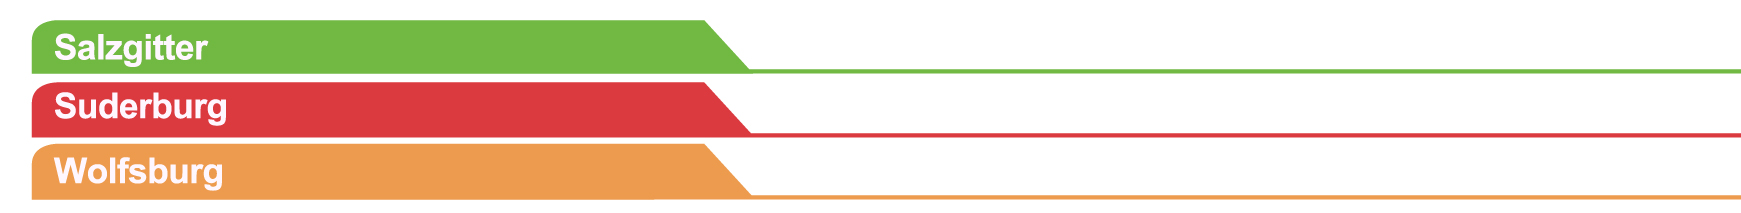
\includegraphics[scale=1.20]{Bilder/reiter_szsudwob_174mm.jpg}
	\end{minipage}
	
	%*******************************************************************************
	
\end{titlepage}
	
	\tableofcontents
	\listoffigures
	\listoftables
	
	\chapter*{Erklärung}

Hiermit versichere ich, dass ich die vorliegende Arbeit selbständig verfasst und keine anderen als die angegebenen Quellen und Hilfsmittel benutzt habe. Ich versichere, dass ich alle wörtlich oder sinngemäß aus anderen Werken übernommenen Aussagen als solche gekennzeichnet habe, und dass die eingereichte Arbeit weder vollständig noch in wesentlichen Teilen Gegenstand eines anderen Prüfungsverfahrens gewesen ist.

\vspace*{3em}

\newcommand*{\SignatureAndDate}[1]{
	\par\noindent\makebox[52mm]{\hrulefill}     \hfill\makebox[65mm]{\hrulefill}
	\par\noindent\makebox[52mm][l]{Ort, Datum}	\hfill\makebox[62mm][l]{#1}
}

\SignatureAndDate{Unterschrift}
	
	\mainmatter
	\chapter{Beispiel}

\section{Das erste Beispiel}

\subsection{Zuerst ein Unterpunkt}
Lorem ipsum dolor sit amet, consectetur adipiscing elit. Aliquam dolor leo, molestie a quam et, egestas tempus augue. Proin adipiscing velit sit amet massa facilisis, in aliquet magna imperdiet. Aenean bibendum ante ut fermentum fermentum. Proin id felis ac nisl pulvinar ornare. Nunc dignissim dignissim turpis. Sed ultricies sit amet ipsum id bibendum. Maecenas adipiscing neque tellus.\footnote{Hallo herzlich Willkommen zu dieser Fußnote.}

Nunc commodo vel dolor non mollis. Duis ac molestie quam, id sagittis tellus. Maecenas iaculis nunc fringilla orci feugiat blandit. Nulla a nibh nec lectus fringilla suscipit. Pellentesque sed mauris vel mauris condimentum rhoncus. Morbi a eros ultrices massa hendrerit viverra ut eget risus. Donec ut enim gravida, lacinia mi sed, faucibus turpis. Duis sagittis arcu tortor, vitae auctor mauris pharetra a. Proin felis justo, scelerisque a augue quis, commodo feugiat ante. Donec consectetur rhoncus leo et auctor. Quisque sit amet fermentum eros. Proin ac tristique dolor, et tincidunt ipsum. Duis semper elit ultricies quam pellentesque, at pharetra augue blandit.

\begin{figure}
	\begin{center}
		
\includegraphics{bilder/ostfalia_logo.jpg}
		\caption{Das Ostfalia Logo. Tada!}
	\end{center}
\end{figure}

\subsubsection{SubSubSection}
Proin non mi sollicitudin, tempus ligula sit amet, congue dui. Suspendisse rutrum tellus porttitor, semper justo et, volutpat lectus. Vestibulum ante ipsum primis in faucibus orci luctus et ultrices posuere cubilia Curae; Ut quis nisi nibh. Ut porttitor egestas nisi in suscipit. Quisque nec tortor eu felis tincidunt tempor nec nec justo. Donec iaculis hendrerit urna, id iaculis sem lobortis tincidunt.

Vestibulum pharetra venenatis nisi, nec venenatis mauris congue at. Phasellus quis vehicula felis. Nam non orci quis nisl suscipit pretium sed id lectus. Etiam ut elementum est. Praesent ultrices nunc nisi, placerat accumsan lorem varius eu. Donec suscipit interdum nunc, at sagittis sem lacinia quis. Nunc adipiscing lacinia magna non lacinia. Integer id euismod enim, quis sagittis massa.

\subsection{Fazit der Subsection}
Lorem ipsum dolor sit amet, consectetur adipiscing elit. Aliquam dolor leo, molestie a quam et, egestas tempus augue. Proin adipiscing velit sit amet massa facilisis, in aliquet magna imperdiet. Aenean bibendum ante ut fermentum fermentum. Proin id felis ac nisl pulvinar ornare. Nunc dignissim dignissim turpis. Sed ultricies sit amet ipsum id bibendum. Maecenas adipiscing neque tellus.

Nunc commodo vel dolor non mollis. Duis ac molestie quam, id sagittis tellus. \cite{Prevezanos2013}  Maecenas iaculis nunc fringilla orci feugiat blandit. Nulla a nibh nec lectus fringilla suscipit. Pellentesque sed mauris vel mauris condimentum rhoncus. Morbi a eros ultrices massa hendrerit viverra ut eget risus. Donec ut enim gravida, lacinia mi sed, faucibus turpis. Duis sagittis arcu tortor, vitae auctor mauris pharetra a. Proin felis justo, scelerisque a augue quis, commodo feugiat ante. Donec consectetur rhoncus leo et auctor. Quisque sit amet fermentum eros. Proin ac tristique dolor, et tincidunt ipsum. Duis semper elit ultricies quam pellentesque, at pharetra augue blandit.

Proin non mi sollicitudin, tempus ligula sit amet, congue dui. Suspendisse rutrum tellus porttitor, semper justo et, volutpat lectus. Vestibulum ante ipsum primis in faucibus orci luctus et ultrices posuere cubilia Curae; Ut quis nisi nibh. Ut porttitor egestas nisi in suscipit. Quisque nec tortor eu felis tincidunt tempor nec nec justo. Donec iaculis hendrerit urna, id iaculis sem lobortis tincidunt.

Vestibulum pharetra venenatis nisi, nec venenatis mauris congue at. Phasellus quis vehicula felis. Nam non orci quis nisl suscipit pretium sed id lectus. Etiam ut elementum est. Praesent ultrices nunc nisi, placerat accumsan lorem varius eu. Donec suscipit interdum nunc, at sagittis sem lacinia quis. Nunc adipiscing lacinia magna non lacinia. Integer id euismod enim, quis sagittis massa.

\begin{table}
	\begin{center}
		\begin{tabular}{| l c r |}
			\hline
			1 & 2 & 3 \\
			4 & 5 & 6 \\
			7 & 8 & 9 \\
			\hline
		\end{tabular}
	\end{center}
	\caption{Ist das nicht eine schöne Tabelle?}
\end{table}

\section{Das zweite Beispiel}

\subsection{Zuerst ein Unterpunkt}
Lorem ipsum dolor sit amet, consectetur adipiscing elit. Aliquam dolor leo, molestie a quam et, egestas tempus augue. Proin adipiscing velit sit amet massa facilisis, in aliquet magna imperdiet. Aenean bibendum ante ut fermentum fermentum. Proin id felis ac nisl pulvinar ornare. Nunc dignissim dignissim turpis. Sed ultricies sit amet ipsum id bibendum. Maecenas adipiscing neque tellus.

Nunc commodo vel dolor non mollis. Duis ac molestie quam, id sagittis tellus. Maecenas iaculis nunc fringilla orci feugiat blandit. Nulla a nibh nec lectus fringilla suscipit. Pellentesque sed mauris vel mauris condimentum rhoncus. Morbi a eros ultrices massa hendrerit viverra ut eget risus. Donec ut enim gravida, lacinia mi sed, faucibus turpis. Duis sagittis arcu tortor, vitae auctor mauris pharetra a. Proin felis justo, scelerisque a augue quis, commodo feugiat ante. Donec consectetur rhoncus leo et auctor. Quisque sit amet fermentum eros. Proin ac tristique dolor, et tincidunt ipsum. Duis semper elit ultricies quam pellentesque, at pharetra augue blandit.

Proin non mi sollicitudin, tempus ligula sit amet, congue dui. Suspendisse rutrum tellus porttitor, semper justo et, volutpat lectus. Vestibulum ante ipsum primis in faucibus orci luctus et ultrices posuere cubilia Curae; Ut quis nisi nibh. Ut porttitor egestas nisi in suscipit. Quisque nec tortor eu felis tincidunt tempor nec nec justo. Donec iaculis hendrerit urna, id iaculis sem lobortis tincidunt.

Vestibulum pharetra venenatis nisi, nec venenatis mauris congue at. Phasellus quis vehicula felis. Nam non orci quis nisl suscipit pretium sed id lectus. Etiam ut elementum est. Praesent ultrices nunc nisi, placerat accumsan lorem varius eu. Donec suscipit interdum nunc, at sagittis sem lacinia quis. Nunc adipiscing lacinia magna non lacinia. Integer id euismod enim, quis sagittis massa.

\subsection{Fazit der Subsection}
Lorem ipsum dolor sit amet, consectetur adipiscing elit. Aliquam dolor leo, molestie a quam et, egestas tempus augue. Proin adipiscing velit sit amet massa facilisis, in aliquet magna imperdiet. Aenean bibendum ante ut fermentum fermentum. Proin id felis ac nisl pulvinar ornare. Nunc dignissim dignissim turpis. Sed ultricies sit amet ipsum id bibendum. Maecenas adipiscing neque tellus.

Nunc commodo vel dolor non mollis. Duis ac molestie quam, id sagittis tellus. Maecenas iaculis nunc fringilla orci feugiat blandit. Nulla a nibh nec lectus fringilla suscipit. Pellentesque sed mauris vel mauris condimentum rhoncus. Morbi a eros ultrices massa hendrerit viverra ut eget risus. Donec ut enim gravida, lacinia mi sed, faucibus turpis. Duis sagittis arcu tortor, vitae auctor mauris pharetra a. Proin felis justo, scelerisque a augue quis, commodo feugiat ante. Donec consectetur rhoncus leo et auctor. Quisque sit amet fermentum eros. Proin ac tristique dolor, et tincidunt ipsum. Duis semper elit ultricies quam pellentesque, at pharetra augue blandit. \cite{Martin:2008:CCH:1388398}

Proin non mi sollicitudin, tempus ligula sit amet, congue dui. Suspendisse rutrum tellus porttitor, semper justo et, volutpat lectus. Vestibulum ante ipsum primis in faucibus orci luctus et ultrices posuere cubilia Curae; Ut quis nisi nibh. Ut porttitor egestas nisi in suscipit. Quisque nec tortor eu felis tincidunt tempor nec nec justo. Donec iaculis hendrerit urna, id iaculis sem lobortis tincidunt.

\lstinputlisting[caption=Some Code,language=Html]{Kapitel/Beispiel/index.html}

Vestibulum pharetra venenatis nisi, nec venenatis mauris congue at. Phasellus quis vehicula felis. Nam non orci quis nisl suscipit pretium sed id lectus. Etiam ut elementum est. Praesent ultrices nunc nisi, placerat accumsan lorem varius eu. Donec suscipit interdum nunc, at sagittis sem lacinia quis. Nunc adipiscing lacinia magna non lacinia. Integer id euismod enim, quis sagittis massa.

\lstinputlisting[caption=Some Code,language=Java]{Kapitel/Beispiel/IntegralTimeProjectMapped.java}

Proin non mi sollicitudin, tempus ligula sit amet, congue dui. Suspendisse rutrum tellus porttitor, semper justo et, volutpat lectus. Vestibulum ante ipsum primis in faucibus orci luctus et ultrices posuere cubilia Curae; Ut quis nisi nibh. Ut porttitor egestas nisi in suscipit. Quisque nec tortor eu felis tincidunt tempor nec nec justo. Donec iaculis hendrerit urna, id iaculis sem lobortis tincidunt.

Vestibulum pharetra venenatis nisi, nec venenatis mauris congue at. Phasellus quis vehicula felis. Nam non orci quis nisl suscipit pretium sed id lectus. Etiam ut elementum est. Praesent ultrices nunc nisi, placerat accumsan lorem varius eu. Donec suscipit interdum nunc, at sagittis sem lacinia quis. Nunc adipiscing lacinia magna non lacinia. Integer id euismod enim, quis sagittis massa.
	\chapter{Beispiel}

\section{Das erste Beispiel}

\subsection{Zuerst ein Unterpunkt}
Lorem ipsum dolor sit amet, consectetur adipiscing elit. Aliquam dolor leo, molestie a quam et, egestas tempus augue. Proin adipiscing velit sit amet massa facilisis, in aliquet magna imperdiet. Aenean bibendum ante ut fermentum fermentum. Proin id felis ac nisl pulvinar ornare. Nunc dignissim dignissim turpis. Sed ultricies sit amet ipsum id bibendum. Maecenas adipiscing neque tellus.\footnote{Hallo herzlich Willkommen zu dieser Fußnote.}

Nunc commodo vel dolor non mollis. Duis ac molestie quam, id sagittis tellus. Maecenas iaculis nunc fringilla orci feugiat blandit. Nulla a nibh nec lectus fringilla suscipit. Pellentesque sed mauris vel mauris condimentum rhoncus. Morbi a eros ultrices massa hendrerit viverra ut eget risus. Donec ut enim gravida, lacinia mi sed, faucibus turpis. Duis sagittis arcu tortor, vitae auctor mauris pharetra a. Proin felis justo, scelerisque a augue quis, commodo feugiat ante. Donec consectetur rhoncus leo et auctor. Quisque sit amet fermentum eros. Proin ac tristique dolor, et tincidunt ipsum. Duis semper elit ultricies quam pellentesque, at pharetra augue blandit.

\begin{figure}
	\begin{center}
		
\includegraphics{bilder/ostfalia_logo.jpg}
		\caption{Das Ostfalia Logo. Tada!}
	\end{center}
\end{figure}

\subsubsection{SubSubSection}
Proin non mi sollicitudin, tempus ligula sit amet, congue dui. Suspendisse rutrum tellus porttitor, semper justo et, volutpat lectus. Vestibulum ante ipsum primis in faucibus orci luctus et ultrices posuere cubilia Curae; Ut quis nisi nibh. Ut porttitor egestas nisi in suscipit. Quisque nec tortor eu felis tincidunt tempor nec nec justo. Donec iaculis hendrerit urna, id iaculis sem lobortis tincidunt.

Vestibulum pharetra venenatis nisi, nec venenatis mauris congue at. Phasellus quis vehicula felis. Nam non orci quis nisl suscipit pretium sed id lectus. Etiam ut elementum est. Praesent ultrices nunc nisi, placerat accumsan lorem varius eu. Donec suscipit interdum nunc, at sagittis sem lacinia quis. Nunc adipiscing lacinia magna non lacinia. Integer id euismod enim, quis sagittis massa.

\subsection{Fazit der Subsection}
Lorem ipsum dolor sit amet, consectetur adipiscing elit. Aliquam dolor leo, molestie a quam et, egestas tempus augue. Proin adipiscing velit sit amet massa facilisis, in aliquet magna imperdiet. Aenean bibendum ante ut fermentum fermentum. Proin id felis ac nisl pulvinar ornare. Nunc dignissim dignissim turpis. Sed ultricies sit amet ipsum id bibendum. Maecenas adipiscing neque tellus.

Nunc commodo vel dolor non mollis. Duis ac molestie quam, id sagittis tellus. \cite{Prevezanos2013}  Maecenas iaculis nunc fringilla orci feugiat blandit. Nulla a nibh nec lectus fringilla suscipit. Pellentesque sed mauris vel mauris condimentum rhoncus. Morbi a eros ultrices massa hendrerit viverra ut eget risus. Donec ut enim gravida, lacinia mi sed, faucibus turpis. Duis sagittis arcu tortor, vitae auctor mauris pharetra a. Proin felis justo, scelerisque a augue quis, commodo feugiat ante. Donec consectetur rhoncus leo et auctor. Quisque sit amet fermentum eros. Proin ac tristique dolor, et tincidunt ipsum. Duis semper elit ultricies quam pellentesque, at pharetra augue blandit.

Proin non mi sollicitudin, tempus ligula sit amet, congue dui. Suspendisse rutrum tellus porttitor, semper justo et, volutpat lectus. Vestibulum ante ipsum primis in faucibus orci luctus et ultrices posuere cubilia Curae; Ut quis nisi nibh. Ut porttitor egestas nisi in suscipit. Quisque nec tortor eu felis tincidunt tempor nec nec justo. Donec iaculis hendrerit urna, id iaculis sem lobortis tincidunt.

Vestibulum pharetra venenatis nisi, nec venenatis mauris congue at. Phasellus quis vehicula felis. Nam non orci quis nisl suscipit pretium sed id lectus. Etiam ut elementum est. Praesent ultrices nunc nisi, placerat accumsan lorem varius eu. Donec suscipit interdum nunc, at sagittis sem lacinia quis. Nunc adipiscing lacinia magna non lacinia. Integer id euismod enim, quis sagittis massa.

\begin{table}
	\begin{center}
		\begin{tabular}{| l c r |}
			\hline
			1 & 2 & 3 \\
			4 & 5 & 6 \\
			7 & 8 & 9 \\
			\hline
		\end{tabular}
	\end{center}
	\caption{Ist das nicht eine schöne Tabelle?}
\end{table}

\section{Das zweite Beispiel}

\subsection{Zuerst ein Unterpunkt}
Lorem ipsum dolor sit amet, consectetur adipiscing elit. Aliquam dolor leo, molestie a quam et, egestas tempus augue. Proin adipiscing velit sit amet massa facilisis, in aliquet magna imperdiet. Aenean bibendum ante ut fermentum fermentum. Proin id felis ac nisl pulvinar ornare. Nunc dignissim dignissim turpis. Sed ultricies sit amet ipsum id bibendum. Maecenas adipiscing neque tellus.

Nunc commodo vel dolor non mollis. Duis ac molestie quam, id sagittis tellus. Maecenas iaculis nunc fringilla orci feugiat blandit. Nulla a nibh nec lectus fringilla suscipit. Pellentesque sed mauris vel mauris condimentum rhoncus. Morbi a eros ultrices massa hendrerit viverra ut eget risus. Donec ut enim gravida, lacinia mi sed, faucibus turpis. Duis sagittis arcu tortor, vitae auctor mauris pharetra a. Proin felis justo, scelerisque a augue quis, commodo feugiat ante. Donec consectetur rhoncus leo et auctor. Quisque sit amet fermentum eros. Proin ac tristique dolor, et tincidunt ipsum. Duis semper elit ultricies quam pellentesque, at pharetra augue blandit.

Proin non mi sollicitudin, tempus ligula sit amet, congue dui. Suspendisse rutrum tellus porttitor, semper justo et, volutpat lectus. Vestibulum ante ipsum primis in faucibus orci luctus et ultrices posuere cubilia Curae; Ut quis nisi nibh. Ut porttitor egestas nisi in suscipit. Quisque nec tortor eu felis tincidunt tempor nec nec justo. Donec iaculis hendrerit urna, id iaculis sem lobortis tincidunt.

Vestibulum pharetra venenatis nisi, nec venenatis mauris congue at. Phasellus quis vehicula felis. Nam non orci quis nisl suscipit pretium sed id lectus. Etiam ut elementum est. Praesent ultrices nunc nisi, placerat accumsan lorem varius eu. Donec suscipit interdum nunc, at sagittis sem lacinia quis. Nunc adipiscing lacinia magna non lacinia. Integer id euismod enim, quis sagittis massa.

\subsection{Fazit der Subsection}
Lorem ipsum dolor sit amet, consectetur adipiscing elit. Aliquam dolor leo, molestie a quam et, egestas tempus augue. Proin adipiscing velit sit amet massa facilisis, in aliquet magna imperdiet. Aenean bibendum ante ut fermentum fermentum. Proin id felis ac nisl pulvinar ornare. Nunc dignissim dignissim turpis. Sed ultricies sit amet ipsum id bibendum. Maecenas adipiscing neque tellus.

Nunc commodo vel dolor non mollis. Duis ac molestie quam, id sagittis tellus. Maecenas iaculis nunc fringilla orci feugiat blandit. Nulla a nibh nec lectus fringilla suscipit. Pellentesque sed mauris vel mauris condimentum rhoncus. Morbi a eros ultrices massa hendrerit viverra ut eget risus. Donec ut enim gravida, lacinia mi sed, faucibus turpis. Duis sagittis arcu tortor, vitae auctor mauris pharetra a. Proin felis justo, scelerisque a augue quis, commodo feugiat ante. Donec consectetur rhoncus leo et auctor. Quisque sit amet fermentum eros. Proin ac tristique dolor, et tincidunt ipsum. Duis semper elit ultricies quam pellentesque, at pharetra augue blandit. \cite{Martin:2008:CCH:1388398}

Proin non mi sollicitudin, tempus ligula sit amet, congue dui. Suspendisse rutrum tellus porttitor, semper justo et, volutpat lectus. Vestibulum ante ipsum primis in faucibus orci luctus et ultrices posuere cubilia Curae; Ut quis nisi nibh. Ut porttitor egestas nisi in suscipit. Quisque nec tortor eu felis tincidunt tempor nec nec justo. Donec iaculis hendrerit urna, id iaculis sem lobortis tincidunt.

\lstinputlisting[caption=Some Code,language=Html]{Kapitel/Beispiel/index.html}

Vestibulum pharetra venenatis nisi, nec venenatis mauris congue at. Phasellus quis vehicula felis. Nam non orci quis nisl suscipit pretium sed id lectus. Etiam ut elementum est. Praesent ultrices nunc nisi, placerat accumsan lorem varius eu. Donec suscipit interdum nunc, at sagittis sem lacinia quis. Nunc adipiscing lacinia magna non lacinia. Integer id euismod enim, quis sagittis massa.

\lstinputlisting[caption=Some Code,language=Java]{Kapitel/Beispiel/IntegralTimeProjectMapped.java}

Proin non mi sollicitudin, tempus ligula sit amet, congue dui. Suspendisse rutrum tellus porttitor, semper justo et, volutpat lectus. Vestibulum ante ipsum primis in faucibus orci luctus et ultrices posuere cubilia Curae; Ut quis nisi nibh. Ut porttitor egestas nisi in suscipit. Quisque nec tortor eu felis tincidunt tempor nec nec justo. Donec iaculis hendrerit urna, id iaculis sem lobortis tincidunt.

Vestibulum pharetra venenatis nisi, nec venenatis mauris congue at. Phasellus quis vehicula felis. Nam non orci quis nisl suscipit pretium sed id lectus. Etiam ut elementum est. Praesent ultrices nunc nisi, placerat accumsan lorem varius eu. Donec suscipit interdum nunc, at sagittis sem lacinia quis. Nunc adipiscing lacinia magna non lacinia. Integer id euismod enim, quis sagittis massa.

	\bibliographystyle{alphadin} 
	\bibliography{literatur}
	
	\clearpage
	\appendix
	\pagenumbering{Roman}
	\chapter{Beispiel}

\section{Das erste Beispiel}

\subsection{Zuerst ein Unterpunkt}
Lorem ipsum dolor sit amet, consectetur adipiscing elit. Aliquam dolor leo, molestie a quam et, egestas tempus augue. Proin adipiscing velit sit amet massa facilisis, in aliquet magna imperdiet. Aenean bibendum ante ut fermentum fermentum. Proin id felis ac nisl pulvinar ornare. Nunc dignissim dignissim turpis. Sed ultricies sit amet ipsum id bibendum. Maecenas adipiscing neque tellus.\footnote{Hallo herzlich Willkommen zu dieser Fußnote.}

Nunc commodo vel dolor non mollis. Duis ac molestie quam, id sagittis tellus. Maecenas iaculis nunc fringilla orci feugiat blandit. Nulla a nibh nec lectus fringilla suscipit. Pellentesque sed mauris vel mauris condimentum rhoncus. Morbi a eros ultrices massa hendrerit viverra ut eget risus. Donec ut enim gravida, lacinia mi sed, faucibus turpis. Duis sagittis arcu tortor, vitae auctor mauris pharetra a. Proin felis justo, scelerisque a augue quis, commodo feugiat ante. Donec consectetur rhoncus leo et auctor. Quisque sit amet fermentum eros. Proin ac tristique dolor, et tincidunt ipsum. Duis semper elit ultricies quam pellentesque, at pharetra augue blandit.

\begin{figure}
	\begin{center}
		
\includegraphics{bilder/ostfalia_logo.jpg}
		\caption{Das Ostfalia Logo. Tada!}
	\end{center}
\end{figure}

\subsubsection{SubSubSection}
Proin non mi sollicitudin, tempus ligula sit amet, congue dui. Suspendisse rutrum tellus porttitor, semper justo et, volutpat lectus. Vestibulum ante ipsum primis in faucibus orci luctus et ultrices posuere cubilia Curae; Ut quis nisi nibh. Ut porttitor egestas nisi in suscipit. Quisque nec tortor eu felis tincidunt tempor nec nec justo. Donec iaculis hendrerit urna, id iaculis sem lobortis tincidunt.

Vestibulum pharetra venenatis nisi, nec venenatis mauris congue at. Phasellus quis vehicula felis. Nam non orci quis nisl suscipit pretium sed id lectus. Etiam ut elementum est. Praesent ultrices nunc nisi, placerat accumsan lorem varius eu. Donec suscipit interdum nunc, at sagittis sem lacinia quis. Nunc adipiscing lacinia magna non lacinia. Integer id euismod enim, quis sagittis massa.

\subsection{Fazit der Subsection}
Lorem ipsum dolor sit amet, consectetur adipiscing elit. Aliquam dolor leo, molestie a quam et, egestas tempus augue. Proin adipiscing velit sit amet massa facilisis, in aliquet magna imperdiet. Aenean bibendum ante ut fermentum fermentum. Proin id felis ac nisl pulvinar ornare. Nunc dignissim dignissim turpis. Sed ultricies sit amet ipsum id bibendum. Maecenas adipiscing neque tellus.

Nunc commodo vel dolor non mollis. Duis ac molestie quam, id sagittis tellus. \cite{Prevezanos2013}  Maecenas iaculis nunc fringilla orci feugiat blandit. Nulla a nibh nec lectus fringilla suscipit. Pellentesque sed mauris vel mauris condimentum rhoncus. Morbi a eros ultrices massa hendrerit viverra ut eget risus. Donec ut enim gravida, lacinia mi sed, faucibus turpis. Duis sagittis arcu tortor, vitae auctor mauris pharetra a. Proin felis justo, scelerisque a augue quis, commodo feugiat ante. Donec consectetur rhoncus leo et auctor. Quisque sit amet fermentum eros. Proin ac tristique dolor, et tincidunt ipsum. Duis semper elit ultricies quam pellentesque, at pharetra augue blandit.

Proin non mi sollicitudin, tempus ligula sit amet, congue dui. Suspendisse rutrum tellus porttitor, semper justo et, volutpat lectus. Vestibulum ante ipsum primis in faucibus orci luctus et ultrices posuere cubilia Curae; Ut quis nisi nibh. Ut porttitor egestas nisi in suscipit. Quisque nec tortor eu felis tincidunt tempor nec nec justo. Donec iaculis hendrerit urna, id iaculis sem lobortis tincidunt.

Vestibulum pharetra venenatis nisi, nec venenatis mauris congue at. Phasellus quis vehicula felis. Nam non orci quis nisl suscipit pretium sed id lectus. Etiam ut elementum est. Praesent ultrices nunc nisi, placerat accumsan lorem varius eu. Donec suscipit interdum nunc, at sagittis sem lacinia quis. Nunc adipiscing lacinia magna non lacinia. Integer id euismod enim, quis sagittis massa.

\begin{table}
	\begin{center}
		\begin{tabular}{| l c r |}
			\hline
			1 & 2 & 3 \\
			4 & 5 & 6 \\
			7 & 8 & 9 \\
			\hline
		\end{tabular}
	\end{center}
	\caption{Ist das nicht eine schöne Tabelle?}
\end{table}

\section{Das zweite Beispiel}

\subsection{Zuerst ein Unterpunkt}
Lorem ipsum dolor sit amet, consectetur adipiscing elit. Aliquam dolor leo, molestie a quam et, egestas tempus augue. Proin adipiscing velit sit amet massa facilisis, in aliquet magna imperdiet. Aenean bibendum ante ut fermentum fermentum. Proin id felis ac nisl pulvinar ornare. Nunc dignissim dignissim turpis. Sed ultricies sit amet ipsum id bibendum. Maecenas adipiscing neque tellus.

Nunc commodo vel dolor non mollis. Duis ac molestie quam, id sagittis tellus. Maecenas iaculis nunc fringilla orci feugiat blandit. Nulla a nibh nec lectus fringilla suscipit. Pellentesque sed mauris vel mauris condimentum rhoncus. Morbi a eros ultrices massa hendrerit viverra ut eget risus. Donec ut enim gravida, lacinia mi sed, faucibus turpis. Duis sagittis arcu tortor, vitae auctor mauris pharetra a. Proin felis justo, scelerisque a augue quis, commodo feugiat ante. Donec consectetur rhoncus leo et auctor. Quisque sit amet fermentum eros. Proin ac tristique dolor, et tincidunt ipsum. Duis semper elit ultricies quam pellentesque, at pharetra augue blandit.

Proin non mi sollicitudin, tempus ligula sit amet, congue dui. Suspendisse rutrum tellus porttitor, semper justo et, volutpat lectus. Vestibulum ante ipsum primis in faucibus orci luctus et ultrices posuere cubilia Curae; Ut quis nisi nibh. Ut porttitor egestas nisi in suscipit. Quisque nec tortor eu felis tincidunt tempor nec nec justo. Donec iaculis hendrerit urna, id iaculis sem lobortis tincidunt.

Vestibulum pharetra venenatis nisi, nec venenatis mauris congue at. Phasellus quis vehicula felis. Nam non orci quis nisl suscipit pretium sed id lectus. Etiam ut elementum est. Praesent ultrices nunc nisi, placerat accumsan lorem varius eu. Donec suscipit interdum nunc, at sagittis sem lacinia quis. Nunc adipiscing lacinia magna non lacinia. Integer id euismod enim, quis sagittis massa.

\subsection{Fazit der Subsection}
Lorem ipsum dolor sit amet, consectetur adipiscing elit. Aliquam dolor leo, molestie a quam et, egestas tempus augue. Proin adipiscing velit sit amet massa facilisis, in aliquet magna imperdiet. Aenean bibendum ante ut fermentum fermentum. Proin id felis ac nisl pulvinar ornare. Nunc dignissim dignissim turpis. Sed ultricies sit amet ipsum id bibendum. Maecenas adipiscing neque tellus.

Nunc commodo vel dolor non mollis. Duis ac molestie quam, id sagittis tellus. Maecenas iaculis nunc fringilla orci feugiat blandit. Nulla a nibh nec lectus fringilla suscipit. Pellentesque sed mauris vel mauris condimentum rhoncus. Morbi a eros ultrices massa hendrerit viverra ut eget risus. Donec ut enim gravida, lacinia mi sed, faucibus turpis. Duis sagittis arcu tortor, vitae auctor mauris pharetra a. Proin felis justo, scelerisque a augue quis, commodo feugiat ante. Donec consectetur rhoncus leo et auctor. Quisque sit amet fermentum eros. Proin ac tristique dolor, et tincidunt ipsum. Duis semper elit ultricies quam pellentesque, at pharetra augue blandit. \cite{Martin:2008:CCH:1388398}

Proin non mi sollicitudin, tempus ligula sit amet, congue dui. Suspendisse rutrum tellus porttitor, semper justo et, volutpat lectus. Vestibulum ante ipsum primis in faucibus orci luctus et ultrices posuere cubilia Curae; Ut quis nisi nibh. Ut porttitor egestas nisi in suscipit. Quisque nec tortor eu felis tincidunt tempor nec nec justo. Donec iaculis hendrerit urna, id iaculis sem lobortis tincidunt.

\lstinputlisting[caption=Some Code,language=Html]{Kapitel/Beispiel/index.html}

Vestibulum pharetra venenatis nisi, nec venenatis mauris congue at. Phasellus quis vehicula felis. Nam non orci quis nisl suscipit pretium sed id lectus. Etiam ut elementum est. Praesent ultrices nunc nisi, placerat accumsan lorem varius eu. Donec suscipit interdum nunc, at sagittis sem lacinia quis. Nunc adipiscing lacinia magna non lacinia. Integer id euismod enim, quis sagittis massa.

\lstinputlisting[caption=Some Code,language=Java]{Kapitel/Beispiel/IntegralTimeProjectMapped.java}

Proin non mi sollicitudin, tempus ligula sit amet, congue dui. Suspendisse rutrum tellus porttitor, semper justo et, volutpat lectus. Vestibulum ante ipsum primis in faucibus orci luctus et ultrices posuere cubilia Curae; Ut quis nisi nibh. Ut porttitor egestas nisi in suscipit. Quisque nec tortor eu felis tincidunt tempor nec nec justo. Donec iaculis hendrerit urna, id iaculis sem lobortis tincidunt.

Vestibulum pharetra venenatis nisi, nec venenatis mauris congue at. Phasellus quis vehicula felis. Nam non orci quis nisl suscipit pretium sed id lectus. Etiam ut elementum est. Praesent ultrices nunc nisi, placerat accumsan lorem varius eu. Donec suscipit interdum nunc, at sagittis sem lacinia quis. Nunc adipiscing lacinia magna non lacinia. Integer id euismod enim, quis sagittis massa.
\end{document}